\chapter{Implementation}
\label{section:implementation}

In this chapter we will implement three different algorithms, all designed to solve the RL problem.
All of the algorithms in this chapter have a different approach to find an optimal solution.
Different extensions will be applied to each of these algorithms that were suggested in other papers.
In the end we will also present a new extension to one of these algorithms.


\section{Deep-Q-Network}

The first algorithm that we will look at is \emph{Deep-Q-Network (DQN)}.
DQN was presented by DeepMind in 2013.
It was \blockquote[{\cite[1]{atari}}]{the first deep learning model to successfully learn control policies directly from high-dimensional sensory input using reinforcement learning}.
In the original paper it was used to learn Atari 2600 games.


DQN is a model-free off-policy algorithm that makes use of the Bellman expectation equation \ref{eq:bellman_exp_q} to create a recursive variant of the action-value function.
It uses the epsilon greedy policy \ref{eq:pi_dash} to deal with exploration.
In the original paper it learns directly from video input by using Convolutional Neural Networks \cite{cnn_wiki}.
In this thesis we will use Feedforward Neural Networks and learn by continuous sensory input such as velocity or position of our model.
The network will be updated every step by stochastic gradient descent minimizing the MSE (\ref{eq:mse}) between a one-step Bellman term, called the label, and the predicted return from the current state, called the prediction.

Another important aspect that made DQN succeed was a technique called \emph{Experience Replay Memory (ERM)}.
When using ERM the agent does not learn directly from the observations after every step, but first stores the entire transition into a replay buffer and then samples a random \emph{minibatch} from this memory after every time step and trains on this data.
The reason that this is important is because consecutive time steps in each episode are often highly correlated and therefore yield a high variance.
Sampling at random from memory breaks this correlation and therefore increases learning performance drastically.
Another aspect that makes ERM better than online learning is that the same transitions can be used more than once for learning, which makes the algorithm more data efficient.


The full algorithm according to the original paper goes as follows:
\begin{algorithm}[H]
  \caption{Deep Q-learning with Experience Replay}
  \label{alg:vanilla_dqn}
  \begin{algorithmic}[1]
  \Statex{Initialize replay memory $D$ to capacity $N$}
  \Statex{Initialize $Q(s,a;\theta)$ arbitrarily.}
	\For{$episode = 1$, $M$}
		\State{Observe initial state $s_1$}
		\For{$t = 1$, $T$}
			\State{With probability $\epsilon$ select a random action $a_t$}
      \State{otherwise select $a_t= max_a Q^*(s_t,a;\theta)$}
      \State{Execute action $a_t$, observe reward $r_t$ and new state $s_{t+1}$}
      \State{Store transition $(s_t, a_t, r_t, s_{t+1})$ in $D$}
      \State{Sample random minibatch of transitions $(s_j, a_j, r_j, s_{j+1})$ from $D$}
      \State{Set $y_j = \begin{cases}
    		r_j                                             ,& \text{  if  } s_t \text{ is terminal}\\
    		r_j + \gamma \max_{a'} Q(s_{j+1}, a'; \theta)   ,& \text{  else  }
    	\end{cases}$}
			\State{Perform a gradient descent step on $(y_j - Q(s_j, a_j; \theta))^2$}
		\EndFor
	\EndFor
  \end{algorithmic}
\end{algorithm}
To understand the behavior of this algorithm, we first tried it on a simpler task than the snake.
The \emph{Cartpole} is a classic RL problem.
The task is to balance a pole on a moving cart by pushing said cart left or right.
The problem here is simplified even further.
The agent can only push by a set amount, meaning that there are two actions every time step.


A known issue with DQN is that it overestimates action values under certain conditions, so the first improvement to the original DQN was to add a so called target network.
The authors of the paper \emph{Deep Reinforcement Learning with Double Q-learning} \cite{ddqn} suggested that adding a second network, called the \emph{target network}, takes care of this issue.
The target network mirrors the original neural net but freezes in time.
This means the original parameters are being copied into the target every few episodes but are not changed otherwise.
The label is then calculated the following way:
\begin{equation} \label{eq:double_label}
	Y_t^{DoubleDQN} = R_{t+1} + \gamma Q(S_{t+1}, \operatorname{arg\,max}_{a}Q(S_{t+1}, a; \theta_t), \theta_t^-)
\end{equation}
Here $\theta$ denotes the variables of the original network while $\theta^-$ denotes the variables of the target network.
Another improvement to the algorithm was adding \emph{Prioritized Experience Replay (PER)} as presented in DeepMind's paper with the same name \cite{per}.
PER improves the already used ERM by not sampling from random but from the importance of a transition.
The importance is defined by how unexpected a transition turned out to be.
Unexpected transition yield more useful training information than expected ones.
In mathematical terms an unexpected transition is one that yields a high TD-Error.
In fact PER introduces \blockquote[{\cite[4]{per}}]{a stochastic sampling method that interpolates between pure greedy prioritization and uniform random sampling.}
The weight change for training is then increased or decreased depending on the importance of the sampled transition.
For performance reasons it is said that implementation should be done by splitting the replay memory into segments of similar importance and then sample one transition from each segment per batch.
Algorithm \ref{alg:ddqn_per} shows the final algorithm we used in this paper for DQN.

\begin{algorithm}[H]
  \caption{Double DQN with proportional prioritization}
  \label{alg:ddqn_per}
  \begin{algorithmic}[1]
  \State{Input: minibatch $k$, step-size $\eta$, replay period $K$ and size $N$, exponents $\alpha$ and $\beta$}
  \State{Initialize replay memory $D$ to capacity $N$}
  \State{Initialize $Q(s,a;\theta)$ arbitrarily.}
  \State{Initialize target $Q_{target}(s,a;\theta')$ arbitrarily.}
  \Let{$\theta'$}{$\theta$}
	\For{$episode = 1$, $M$}
		\State{Observe initial state $s_1$}
		\For{$t = 1$, $T$}
			\State{With probability $\epsilon$ select a random action $a_t$}
      \State{otherwise select $a_t= max_a Q(s_t,a;\theta)$}
      \State{Execute action $a_t$, observe reward $r_t$ and new state $s_{t+1}$}
      \State{Store transition $(s_t, a_t, r_t, s_{t+1})$ in $D$ with maximal priority $p_t = \max_{i<t}p_i$}
      \If{$t \pmod{K} \equiv 0$}
        \For{$j = 1, k$}
          \State{Sample transition $j \sim P(j) = \frac{p_j^\alpha}{\sum_i p_i^\alpha}$}
          \State{Compute importance-sampling weight $w_j = \frac{(N \cdot P(j))^{-\beta}}{\max_i w_i}$}
          \State{$\delta_j = r_{j} + \gamma Q_{target}(s_{j+1}, \operatorname{arg\,max}_{a'} Q(s_{j+1}, a'; \theta); \theta') - Q(s_{j}, a_{j}; \theta)$}
          \Let{$p_j$}{$|\delta_j|$}
          \Let{$\Delta$}{$\Delta + w_{j} \cdot \delta_{j} \cdot \nabla_\theta Q(s_{j}, a_{j}; \theta)$}
        \EndFor
        \Let{$\theta$}{$\theta + \eta \cdot \Delta$}
        \Let{$\Delta$}{$0$}
        \State{From time to time copy weights into target network $\theta' \leftarrow \theta$}
      \EndIf
		\EndFor
	\EndFor
  \end{algorithmic}
\end{algorithm}

The last improvement that was made to the DQN was presented in the paper \emph{Dueling Network Architectures for Deep Reinforcement Learning (Wang et al.)} \cite{duel_dqn}.
They present a network architecture that can deal with different necessities of estimating the value for each action in a state.
Take the Cartpole as an example, if the pole is straight it doesn't matter whether the cart pushes left or right.
But it becomes really important if the pole is about to fall to far in a certain direction.


In mathematical terms this insight is realized by splitting the single streamed feedforward network into two sequences.
While one stream will estimate the value function $V(s)$, the other will estimate the advantage function $A(s,a)$.
In the end both are added back together to result into the action value function estimate.
Equation \ref{eq:duel_dqn} shows how both streams are added back up to result into the action-value function $Q(s,a)$.
\begin{equation} \label{eq:duel_dqn}
  Q(s,a) = V(s) + A(s,a) - \frac{1}{|A|}\sum_{a'}A(s,a)
\end{equation}
Note that the target network will be modified the same way.


Figure \ref{eq:duel_dqn} shows the new network architecture for our Dueling-Double-DQN and listing \ref{lst:duel-net} is the corresponding Python code.

\begin{center}
\begin{tikzpicture}[node distance=0cm]
\label{fig:duel_dqn}

\node (init) {};

\node [block_big] (mlp) {\LARGE Neural Net};

\node [right= 2cm of mlp] (dummy) {};
\node [round, above= 0.5cm of dummy] (1) {};
\node [round, above= 0.5cm of 1] (2) {};
\node [round, above= 0.5cm of 2] (3) {};
\node [text width=3cm, text centered] at ($(3) + (0.0,1.0)$) {Value Part};

\node [round, below= 0.5cm of dummy] (4) {};
\node [round, below= 0.5cm of 4] (5) {};
\node [round, below= 0.5cm of 5] (6) {};
\node [text width=3cm, text centered] at ($(6) + (0.0,-1.0)$) {Advantage Part};

\node [round, right= 2em of 2] (7) {$V(S)$};
\node [round] (8) at ($(4)!0.5!(5) + (1.66,0.0)$) {$A_1$};
\node [round] (9) at ($(5)!0.5!(6) + (1.66,0.0)$) {$A_2$};

\node [round_big] (mean) at ($(8)!0.5!(9) + (2.0,0.0)$) {\Large $\frac{1}{N}\Sigma$};

\node [round_big, right= 7cm of mlp] (minus) {\LARGE $-$};

\node [right=1cm of minus] (q) {$Q(S,A)$};


\path [line] (mlp) -- (1);
\path [line] (mlp) -- (2);
\path [line] (mlp) -- (3);
\path [line] (mlp) -- (4);
\path [line] (mlp) -- (5);
\path [line] (mlp) -- (6);

\path [line] (1) -- (7);
\path [line] (2) -- (7);
\path [line] (3) -- (7);
\path [line] (4) -- (8);
\path [line] (5) -- (8);
\path [line] (6) -- (8);
\path [line] (4) -- (9);
\path [line] (5) -- (9);
\path [line] (6) -- (9);

\path [line] (8) -- (mean);
\path [line] (9) -- (mean);

\path [line] (mean) -- (minus);
\path [line] (7) -- (minus);

\path [line] (minus) -- (q);


\end{tikzpicture}
\captionof{figure}{Conceptual view of the dueling Q-Network}
\end{center}

\begin{lstlisting}[language=Python, caption=Python code for the dueling network, captionpos=b, label=lst:duel-net]
#The first hidden layer stays the same
hidden1 = tf.layers.dense(input_pl, hidden1_size, tf.nn.relu)
#Now the stream is split into two
value = tf.layers.dense(hidden1, 1, tf.nn.relu)
advantage = tf.layers.dense(hidden1, output_size, tf.nn.relu)
#And added back together
output = tf.add(value, tf.subtract(advantage,
  tf.reduce_mean(advantage, axis=1, keep_dims=True)))
\end{lstlisting}

\section{Deep Deterministic Policy Gradient}

The second algorithm we use was presented by Lillicrap et al. in the paper \emph{Continuous control with deep reinforcement learning} \cite{ddpg}.
\emph{Deep Deterministic Policy Gradient} or short DDPG takes many aspects of DQN but applies them to suit continuous action domains.
DDPG is \blockquote[{\cite[1]{ddpg}}]{an actor-critic, model-free algorithm based on the deterministic policy gradient that can operate over continuous action spaces.}
The algorithm makes use of the \emph{Deterministic Policy Gradient Theorem} (\ref{eq:d_p_g_theorem}) but combines it with insights of the success of DQN.
As in DQN DDPG does not learn directly from observations but stores transitions into an ERM to break the correlation between different observations.
At every time step a minibatch is sampled from memory to train the networks.
It also uses target networks, but instead of doing hard copies of the original into the target, it performs soft updates every time step using an exponential filter-like updating function.
Equation \ref{eq:ddpg_update} shows such a soft update.

\begin{align}
  \label{eq:ddpg_update}
  \theta^Q \leftarrow \tau \theta^Q + (1 - \tau) \theta^{Q'} \nonumber\\
  \theta^\mu \leftarrow \tau \theta^\mu + (1 - \tau) \theta^{\mu'}
\end{align}
where $\theta^Q$ are the parameters of the Q-function, $\theta^\mu$ are the parameters of the policy and $\tau$ is an update rate.
DDPG uses the critic to approximate the Q-value function while the actor approximates the policy.
The critic is updated just like the DQN with a one-step Bellman term as the label, the output of the network as our prediction and MSE as the loss function.
The actor is then updated by calculating the critic's gradient regarding the actions and multiplying it with the gradient of the actor regarding its parameters.
This is exactly as stated in the \emph{Deterministic Policy Gradient Theorem} (\ref{eq:d_p_g_theorem}).


In the original paper exploration is achieved by adding noise to the predicted action.
Equation \ref{eq:ac_noise} shows the policy of DDPG when adding noise to it.

\begin{equation}
  \label{eq:ac_noise}
  a_t = \mu(s_t | \theta^\mu) + \mathcal{N}_t
\end{equation}

where $a_t$ is the calculated action, $\mu(s_t | \theta^\mu)$ is the policy evaluation in state $s_t$ and $\mathcal{N}_t$ is some kind of noise generator.
In this thesis we used an Ornstein–Uhlenbeck process to generate our noise that updates its noise state every time step.

\begin{equation}
  dx_t = \theta (\mu - x-t)dt + \sigma d W_t
\end{equation}

where we chose $\theta = 0.15$, $\mu = 0$ and $\sigma = 0.2$ and $dW_t$ to be a uniform random distribution between $0$ and $1$.
The noise state in time step $t+1$ is simply $x_{t+1} = x_t + dx_t$.

While writing this thesis, Plappert et al. introduced a new way to deal with exploration in RL by adding the noise directly to the parameters of the network instead of adding it to the action space \cite{param_noise}.
Equation \ref{eq:param_noise} shows how the parameter noise is introduced.

\begin{equation}
  \label{eq:param_noise}
  \widetilde \theta = \theta + \mathcal{N}(0, \sigma^2 I)
\end{equation}

As one can see it is very similar to \ref{eq:ac_noise} but instead of adding the noise to the policy we now add it to our parameters.

\begin{algorithm}[H]
  \caption{Deep Deterministic Policy Gradient}
  \label{alg:ddpg}
  \begin{algorithmic}[1]
  \State{Initialize replay memory $R$}
  \State{Initialize $Q(s,a | \theta^{Q})$ and $\mu(s | \theta^{\mu})$ arbitrarily.}
  \State{Initialize targets $Q'$ and $\mu'$}
  \Let{$\theta^{Q'}$}{$\theta^Q$}
  \Let{$\theta^{\mu'}$}{$\theta^\mu$}
	\For{$episode = 1$, $M$}
    \State{Initialize a random process $\mathcal{N}$ for exploration}
		\State{Observe initial state $s_1$}
		\For{$t = 1$, $T$}
			\State{Select action $a_t= \mu(s_t | \theta^\mu)$ according to policy and noise state}
      \State{Execute action $a_t$, observe reward $r_t$ and new state $s_{t+1}$}
      \State{Store transition $(s_t, a_t, r_t, s_{t+1})$ in $R$}
      \State{Sample a random minibatch of $N$ transitions $(s_t, a_t, r_t, s_{t+1})$ from $R$}
      \State{Update critic by minimizing $L = \frac{1}{N} \sum_i (y_i - Q(s_i,a_i | \theta^Q))^2$}
      \State{Update the actor's policy using sampled policy gradient:}
      \State{$\displaystyle{\nabla_{\theta^\mu}J \approx \frac{1}{N} \sum_i \nabla_a Q(s,a | \theta^Q)|_{s=s_i, a=\mu(s_i)} \nabla_{\theta^\mu} \mu(s | \theta^\mu)|_{s_i}}$}
      \State{Update the target networks}
      \Let{$\theta^Q$}{$\tau \theta^Q + (1 - \tau) \theta^{Q'}$}
      \Let{$\theta^\mu$}{$\tau \theta^\mu + (1 - \tau) \theta^{\mu'}$}
		\EndFor
	\EndFor
  \end{algorithmic}
\end{algorithm}

Two different network architectures were used for both the actor and the critic.
While the actor's network is a simple feedforward net with two hidden layers, it was found that introducing the action only on the second layer of the critic's network, better results could be obtained.
Listing \ref{lst:ddpg-net} displays the TF code for both networks.

\begin{lstlisting}[language=Python, caption=Python code for the DDPG networks, captionpos=b, label=lst:ddpg-net]
#The actor network
hidden1 = tf.layers.dense(input_pl, hidden1_size, tf.nn.relu)
hidden2 = tf.layers.dense(hidden1, hidden2_size, tf.nn.relu)
output = tf.layers.dense(hidden2, action_space, tf.nn.tanh)
#The critic network
hidden1 = tf.layers.dense(input_pl, hidden1_size, tf.nn.relu)
hidden = tf.layers.dense(hidden1, hidden2_size)
action = tf.layers.dense(action_pl, hidden2_size)
hidden2 = tf.nn.relu(hidden + action)
output = tf.layers.dense(hidden2, 1, tf.nn.tanh)
\end{lstlisting}


\section{Proximal Policy Optimization}

The last kind of algorithm we will use to solve the snake problem was only released while writing this paper.
\emph{Proximal Policy Optimization Algorithms} \cite{ppo}, a paper from the OpenAI team, presents a new class of algorithms for RL.
It builds upon the previously released \emph{Trust Region Policy Optimization} (TRPO) which will not be explained here.
Different to DQN and DDPG, PPO runs its policy for many time steps before updating its parameters with the gathered information.
This drastically decreases the computational costs for the algorithm and we will see that it does not require many more time steps to learn.

PPO's predecessors make use of the \emph{Policy Gradient Theorem} (\ref{eq:p_g_theorem}) but reshape it in a few ways.
Again the objective function $J(\theta)$ will be the same as in Equation \ref{eq:j_theta} but it will make use of two useful identities shown in Equation \ref{eq:j_theta_2}.
\begin{align}
	\label{eq:j_theta_2}
	J(\theta) &= \mathbb{E}_{r \sim \pi} \Big[\sum_t \gamma^t r_t\Big] \nonumber\\
  		      &= \mathbb{E}_{s \sim \pi, a \sim \pi}\Big[A^{\pi_{old}}(s,a)\Big] \nonumber\\
  		      &= \mathbb{E}_{s \sim \pi_{old}, a \sim \pi_{old}}\bigg[\frac{\pi(a | s)}{\pi_{old}(a | s)} A^{\pi_{old}}(s,a)\bigg]
\end{align}
where $\pi_{old}$ is some old policy from which we sample our actions and $A^{\pi_{old}}(s,a)$ are the advantages retrieved under the old policy.
We now define the probability ratio.
\begin{defn}[Probability Ratio]
\begin{equation} \label{eq:prob_ratio_r}
	r_t(\theta) \coloneqq \frac{\pi(a | s)}{\pi_{old}(a | s)}
\end{equation}
\end{defn}
Using \ref{eq:j_theta_2}, Equation \ref{eq:l_cpi} defines a so called \emph{surrogate objective function} which is a local approximation to $J(\theta)$ and will be maximized during learning using stochastic gradient ascent.
\begin{equation} \label{eq:l_cpi}
	L(\theta) = \hat{\mathbb{E}}_{t}\Big[r_t(\theta) \hat{A}_t\Big]
\end{equation}
where $\hat{A}_t$ is an estimator of the advantage function at time step $t$.
In words $L(\theta)$ tries to approximate how much better our new policy is compared to our old one.


Unfortunately maximizing this surrogate can lead to excessively large policy updates which can break the learning process.
This is where PPO proposes a new surrogate objective function depicted in Equation \ref{eq:l_clip}.
\begin{equation} \label{eq:l_clip}
	L^{CLIP}(\theta) = \hat{\mathbb{E}}_{t}\bigg[\min \Big(r_t(\theta) \hat{A}_t, \operatorname*{clip}(r_t(\theta), 1 - \epsilon, 1 + \epsilon) \hat{A}_t \Big)\bigg]
\end{equation}
where $\epsilon$ is a new hyperparameter that defines how heavy the clipping is.
$L^{CLIP}$ takes the minimum of the clipped and unclipped surrogate and therefore reduces the risk of too drastic policy updates.


To approximate the advantage function \emph{General Advantage Estimation} (GAE) is used.
GAE defined in three steps.
First a delta is defined as shown in Equation \ref{eq:gae_delta}.
\begin{defn}[$\delta$ for GAE]
\begin{equation}
  \label{eq:gae_delta}
  \delta_t^V \coloneqq r_t + \gamma V(s_{t+1}) - V(s_t)
\end{equation}
\end{defn}

Then the sum of these $\delta$ terms is denoted as $\hat{A}_t^{k}$, as shown in Equation \ref{eq:gae_ahat}.

\begin{defn}
\begin{equation}
  \label{eq:gae_ahat}
  \hat{A}_t^{(k)} \coloneqq \sum_{l=0}^{k-1} \gamma^l \delta_{t+l}^V
\end{equation}
\end{defn}

At last GAE is defined as the exponentially-weighted average of these estimators.
Equation \ref{eq:gae} shows the full \emph{General Advantage Estimation}.

\begin{defn}[General Advantage Estimation]
\begin{equation}
  \label{eq:gae}
  \hat{A}_t^{GAE(\gamma,\lambda)} \coloneqq \sum_{l=0}^{\infty}(\gamma \lambda)^l \delta_{t+l}^V
\end{equation}
\end{defn}

With this estimator, Equation \ref{eq:l_clip} can be rewritten to include GAE.

\begin{equation}
  \label{eq:l_clip_GAE}
	L^{CLIP}(\theta) = \hat{\mathbb{E}}_{t}\bigg[\min \Big(r_t(\theta) \hat{A}_t^{GAE(\gamma,\lambda)}, \operatorname*{clip}(r_t(\theta), 1 - \epsilon, 1 + \epsilon) \hat{A}_t^{GAE(\gamma,\lambda)} \Big)\bigg]
\end{equation}

Algorithm \ref{alg:ppo} shows the pseudo-code of the PPO we used in this thesis.

\begin{algorithm}[H]
  \caption{Proximal Policy Optimization}
  \label{alg:ppo}
  \begin{algorithmic}[1]
  \State{Initialize replay memory $R$}
  \State{Initialize critic $V(s,a | \theta^{V})$ and  actor $\pi(s | \theta^{\pi})$ arbitrarily.}
	\For{$trajectory = 1$, $M$}
    \State{Initialize a random process $\mathcal{N}$ for exploration}
		\State{Observe initial state $s_1$}
		\For{$timestep = 1$, $T$}
			\State{Select action $a_t= \pi_{\theta_{old}}$ according to policy and noise state}
      \State{Execute action $a_t$, observe reward $r_t$ and new state $s_{t+1}$}
      \State{Store transition $(s_t, a_t, r_t, s_{t+1})$ in $R$}
		\EndFor
    \State{Compute targets $\hat{V}_1$, $\hat{V}_2$, ..., $\hat{V}_T$ from transitions in $R$}
    \State{Compute advantage estimates $\hat{A}_1$, $\hat{A}_2$, ..., $\hat{A}_T$ from transitions in $R$}
    \State{Update actor by performing a gradient ascent step to maximize $L$}
    \State{Update critic by minimizing MSE between $\hat{V}_t$ and $V_t$}
    \State{Clear $R$}
	\EndFor
  \end{algorithmic}
\end{algorithm}

In this thesis we will also try a new approach to exploration.
We will try to change the standard deviation of our policy-distribution to increase or decrease exploration.
Figure \ref{fig:normal_plot} shows how the different standard deviations affect the distribution from which we sample our actions from.
As one can see an increase in $\sigma$ corresponds to a higher chance of picking actions further away from the mean.
We will try different approaches to this idea.
The first approach will be to set $\sigma$ to a specific value.
The second approach will be to uniformly sample $\sigma \in [0.5,1.5]$ before every trajectory.
The third approach will be to use another normal distribution to sample $\sigma$ from before every trajectory.

\begin{figure}[H]
\centerline{
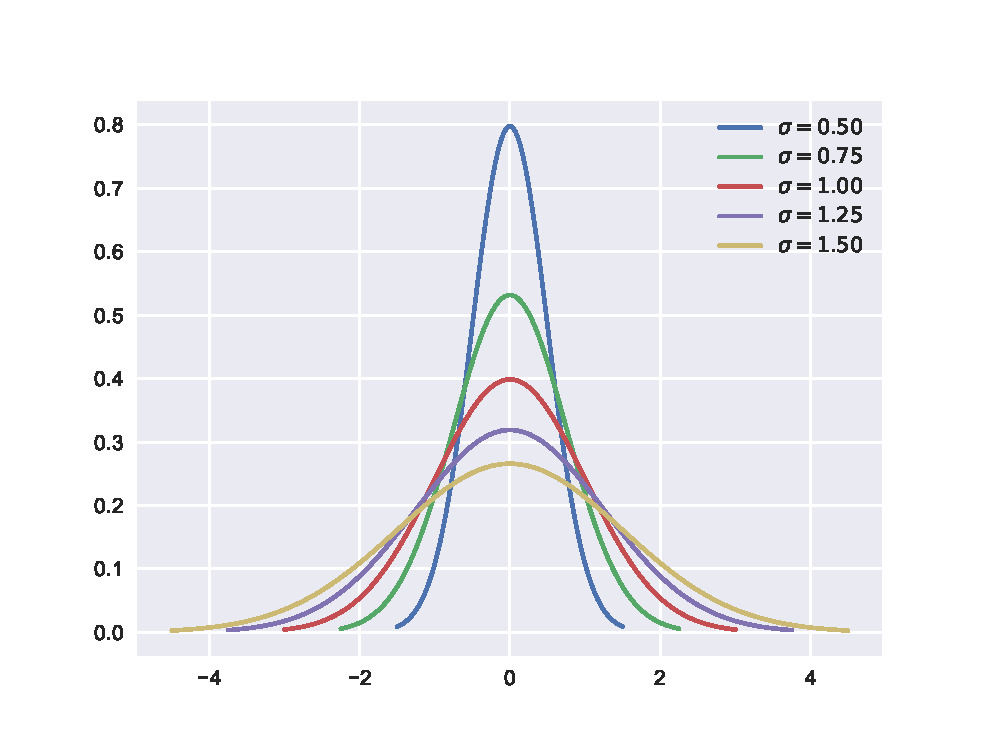
\includegraphics[width=0.7\textwidth]{images/normalPlot.eps}}
\caption{Normal distribution with different standard deviations}
\label{fig:normal_plot}
\end{figure}



In this chapter we looked at three different kinds of algorithms each designed to solve the RL problem.
We presented many extensions to each of these algorithms and in the end presented a new approach also.
In the next chapter we will look at how all of these algorithms performed on different tasks to eventually solve the snake simulation.
